\subsubsection{Objetivo y Enfoque del Sistema de Clasificación}

El sistema de clasificación tiene como objetivo determinar la presencia o ausencia de lechuga en cada estación de cultivo para orientar las decisiones de cosecha. A diferencia de métodos basados en aprendizaje profundo que requieren extensos conjuntos de entrenamiento y elevada capacidad computacional, se implementó un enfoque basado en análisis morfológico y clasificación por umbral estadístico.

La selección de este enfoque se fundamentó en varios criterios. Primero, el costo computacional del análisis morfológico es significativamente menor que el de redes neuronales convolucionales, permitiendo su ejecución en tiempo real sobre la plataforma Raspberry Pi 4 sin necesidad de aceleradores de hardware especializados. Segundo, el método no requiere un extenso dataset etiquetado para entrenamiento, sino únicamente una muestra representativa para establecer parámetros estadísticos. Tercero, el sistema presenta alta interpretabilidad, con parámetros ajustables y verificables que facilitan la depuración y optimización. Finalmente, la precisión alcanzada por este método resulta suficiente para la aplicación, superando el 95 por ciento de exactitud según se demostrará posteriormente.

\subsubsection{Fundamento de la Segmentación Cromática}

El sistema explota el contraste cromático entre las lechugas, que presentan tonalidades verdes características, y el entorno del sistema hidropónico, dominado por superficies blancas y grises de los tubos de PVC y la estructura. Este contraste permite segmentar efectivamente las regiones de vegetación mediante umbralización en el espacio de color HSV.

La segmentación se realiza definiendo un rango de valores en los tres canales del espacio HSV que corresponde a las tonalidades verdes de las lechugas hidropónicas. Cada píxel de la imagen se evalúa individualmente: si sus componentes de matiz, saturación y valor se encuentran dentro de los límites establecidos, el píxel se marca como perteneciente a vegetación; en caso contrario, se marca como fondo. Esta operación genera una máscara binaria donde las regiones blancas corresponden a vegetación detectada y las regiones negras corresponden al resto de la escena.

Los límites del rango cromático se establecieron empíricamente mediante análisis de muestras representativas de lechugas en diferentes estados de desarrollo bajo las condiciones de iluminación del invernadero. El canal de matiz se acotó entre 25 y 85 grados, rango que cubre desde verdes amarillentos hasta verdes azulados, abarcando la variabilidad natural de las lechugas hidropónicas. El límite inferior de saturación se estableció en 40 para eliminar colores desaturados del fondo que podrían presentar componente verde débil. El límite inferior de valor se fijó en 40 para descartar sombras muy oscuras que no corresponden a vegetación iluminada.

La fundamentación teórica de esta estrategia se presentó en la Sección 2.2.1 del marco teórico, donde se demostró que el espacio HSV proporciona robustez ante variaciones de iluminación al separar la información cromática de la información de luminosidad. Esta propiedad resulta crítica en el entorno del invernadero, donde la intensidad luminosa varía significativamente durante el día debido a la luz natural complementaria.

\begin{figure}[H]
\centering
\begin{subfigure}[b]{0.48\textwidth}
    \centering
    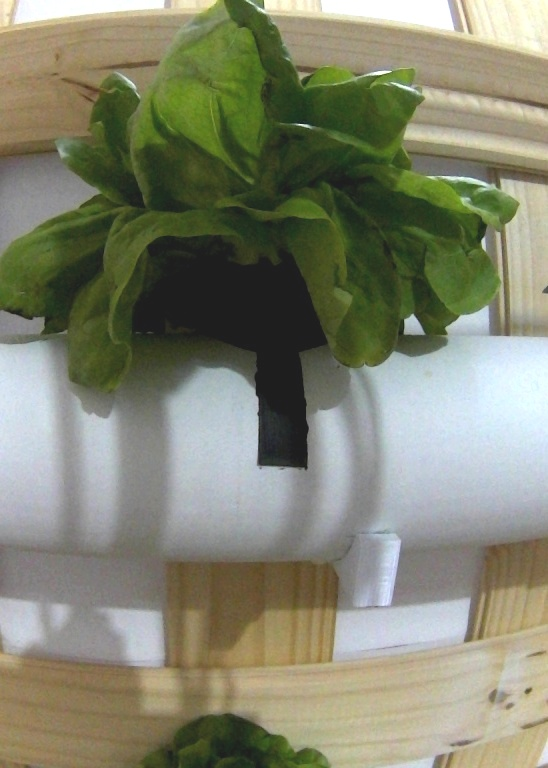
\includegraphics[width=\textwidth]{imagenes/clasificador_1_original.jpg}
    \caption{Imagen RGB original}
\end{subfigure}
\hfill
\begin{subfigure}[b]{0.48\textwidth}
    \centering
    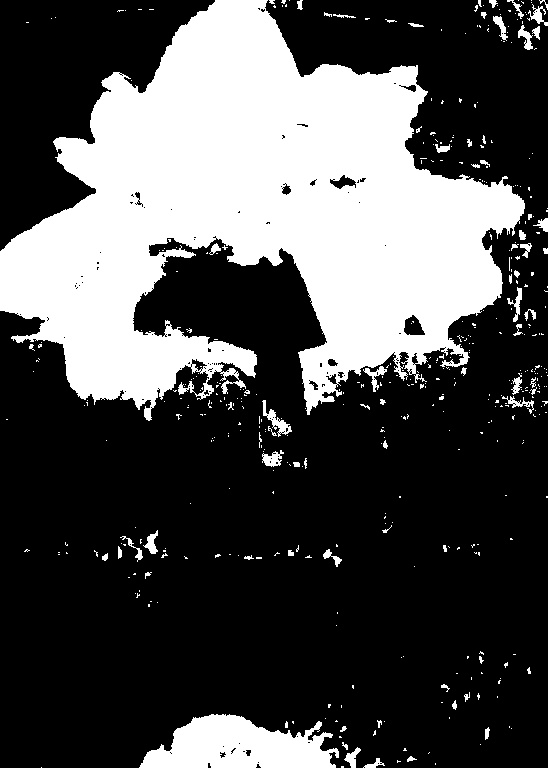
\includegraphics[width=\textwidth]{imagenes/clasificador_2_verde.jpg}
    \caption{Máscara de vegetación verde}
\end{subfigure}
\caption{Proceso de segmentación cromática para detección de vegetación en espacio HSV}
\label{fig:segmentacion_cromatica}
\end{figure}

\subsubsection{Refinamiento de la Máscara de Segmentación}

La máscara binaria resultante de la segmentación cromática presenta típicamente imperfecciones causadas por variaciones locales de iluminación, reflexiones especulares sobre superficies húmedas, y limitaciones inherentes del sensor. Estas imperfecciones se manifiestan como pequeños huecos dentro de las regiones de vegetación y píxeles aislados erróneamente clasificados como vegetación.

Para refinar la máscara se aplica una secuencia de operaciones morfológicas fundamentadas en la teoría presentada en la Sección 2.2.1. La primera operación es el cierre morfológico, que consiste en una dilatación seguida de una erosión con el mismo elemento estructurante. Esta operación rellena huecos pequeños dentro de las regiones y conecta componentes próximos que pudieron haberse fragmentado durante la segmentación. La segunda operación es la apertura morfológica, consistente en una erosión seguida de una dilatación, que elimina píxeles aislados y pequeñas protuberancias que corresponden a ruido.

El elemento estructurante empleado es una matriz rectangular de 3×3 píxeles con todos sus elementos igual a uno. Este tamaño representa un compromiso entre la capacidad de eliminación de ruido y la preservación de detalles relevantes de la forma de las lechugas. Elementos estructurantes mayores eliminarían ruido más efectivamente pero podrían suavizar excesivamente los bordes y eliminar detalles morfológicos importantes.

El resultado del refinamiento morfológico es una máscara donde las regiones de vegetación presentan fronteras más suaves y mayor conectividad interna, facilitando la subsecuente detección de contornos y reduciendo la probabilidad de fragmentación artificial de una lechuga en múltiples componentes.

\subsubsection{Detección y Filtrado de Contornos}

Sobre la máscara refinada se ejecuta el algoritmo de detección de contornos de Suzuki-Abe, aplicando los principios descritos en la Sección 2.2.2 del marco teórico. Este algoritmo identifica las fronteras entre las regiones de vegetación (blancas) y el fondo (negro), generando una representación vectorial de cada contorno como secuencia ordenada de coordenadas de píxeles.

Se emplea el modo de extracción de contornos externos únicamente, dado que las lechugas no presentan huecos internos relevantes para la clasificación. La aproximación de contornos se realiza mediante compresión de segmentos colineales, reduciendo significativamente el uso de memoria sin pérdida de información geométrica esencial.

Los contornos detectados se someten a filtrado para eliminar aquellos que no corresponden a lechugas. El criterio principal de filtrado es el área, calculada como el número de píxeles encerrados por el contorno. Se establece un umbral mínimo de 5000 píxeles, descartando contornos con áreas inferiores que típicamente corresponden a ruido residual, pequeñas sombras o reflexiones.

La justificación de este umbral se basa en consideraciones geométricas. A la distancia de trabajo nominal de 200 milímetros, la resolución espacial es de aproximadamente 0.146 mm/píxel. Un contorno de 5000 píxeles corresponde a un área física de aproximadamente:

\begin{equation}
A_{física} = 5000 \text{ px} \times (0.146 \text{ mm/px})^2 \approx 106 \text{ mm}^2
\end{equation}

Las lechugas en estado mínimo para cosecha presentan diámetros de aproximadamente 50 milímetros, resultando en áreas de aproximadamente:

\begin{equation}
A_{lechuga} = \pi \left(\frac{50}{2}\right)^2 \approx 1963 \text{ mm}^2
\end{equation}

Esta área es significativamente mayor que el umbral de 106 mm², garantizando que las lechugas de interés no sean filtradas inadvertidamente. Por otro lado, elementos espurios como pequeñas sombras o residuos vegetales presentan típicamente áreas inferiores al umbral y son correctamente eliminados.

\subsubsection{Extracción del Descriptor de Área}

De los contornos que superan el filtrado inicial, se selecciona el contorno de mayor área bajo la hipótesis de que la lechuga constituye el objeto verde dominante en la escena cuando está presente. Esta selección se realiza simplemente identificando el contorno cuya área calculada es máxima entre todos los contornos válidos.

El área del contorno seleccionado se calcula mediante el algoritmo de conteo de píxeles interiores empleando el método de relleno por escaneo de líneas, implementado eficientemente en la biblioteca OpenCV. Este valor de área en píxeles constituye el descriptor único empleado para la clasificación.

La decisión de emplear únicamente el área como descriptor se fundamenta en su alto poder discriminativo, demostrado mediante el análisis estadístico que se presenta en la siguiente sección. Otros descriptores geométricos como circularidad, solidez o relación de aspecto podrían proporcionar información complementaria, pero el análisis preliminar reveló que no mejoran significativamente la precisión de clasificación dado el alto grado de separabilidad que proporciona el área por sí sola.

Cuando no se detectan contornos válidos (ningún contorno supera el umbral de área mínima), el sistema concluye que no hay vegetación presente en la imagen y clasifica la estación como vaso vacío con alta confianza. Este caso ocurre naturalmente cuando el vaso está efectivamente vacío o cuando las condiciones de iluminación son tan deficientes que la segmentación cromática no logra identificar vegetación.

\subsubsection{Casos Especiales y Manejo de Ambigüedades}

El sistema implementa lógica específica para manejar casos especiales que podrían comprometer la confiabilidad de la clasificación. Cuando se detectan múltiples contornos grandes (más de tres contornos con área superior a 5000 píxeles), el sistema genera una advertencia indicando posible error de segmentación. Esto podría ocurrir si la iluminación genera sombras fuertes que fragmentan artificialmente la imagen de la lechuga, o si existen elementos extraños en el campo de visión. En estos casos, el sistema procede seleccionando el contorno de mayor área, pero reduce el índice de confianza asociado a la clasificación.

Cuando el área del contorno principal se encuentra en una zona de incertidumbre cercana al umbral de decisión (este concepto se desarrollará en la siguiente sección), el sistema reduce igualmente la confianza de la clasificación. Esta información de confianza puede emplearse en el nivel supervisor para implementar estrategias de verificación adicional, como captura de una segunda imagen desde un ángulo ligeramente diferente.

El tiempo total de procesamiento del pipeline de clasificación, incluyendo captura, conversión HSV, segmentación, morfología, detección de contornos y cálculo de área, es de aproximadamente 143 milisegundos. Esta latencia permite una frecuencia de operación superior a 6 Hz, aunque en la práctica la clasificación se ejecuta únicamente cuando el robot se encuentra estacionado frente a una estación, sin restricciones temporales estrictas.

\begin{figure}[H]
\centering
\begin{subfigure}[b]{0.48\textwidth}
    \centering
    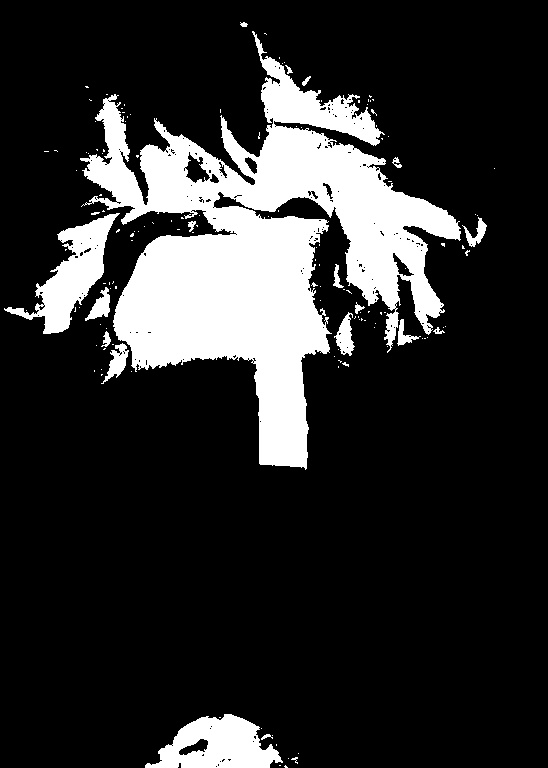
\includegraphics[width=\textwidth]{imagenes/clasificador_3_negro.jpg}
    \caption{Máscara de regiones oscuras}
\end{subfigure}
\hfill
\begin{subfigure}[b]{0.48\textwidth}
    \centering
    
\includegraphics[width=\textwidth]{imagenes/clasificador_4_combinado.jpg}
    \caption{Combinación verde + negro}
\end{subfigure}

\vspace{0.3cm}

\begin{subfigure}[b]{0.48\textwidth}
    \centering
    
\includegraphics[width=\textwidth]{imagenes/clasificador_5_binario_final.jpg}
    \caption{Máscara binaria refinada}
\end{subfigure}
\hfill
\begin{subfigure}[b]{0.48\textwidth}
    \centering
    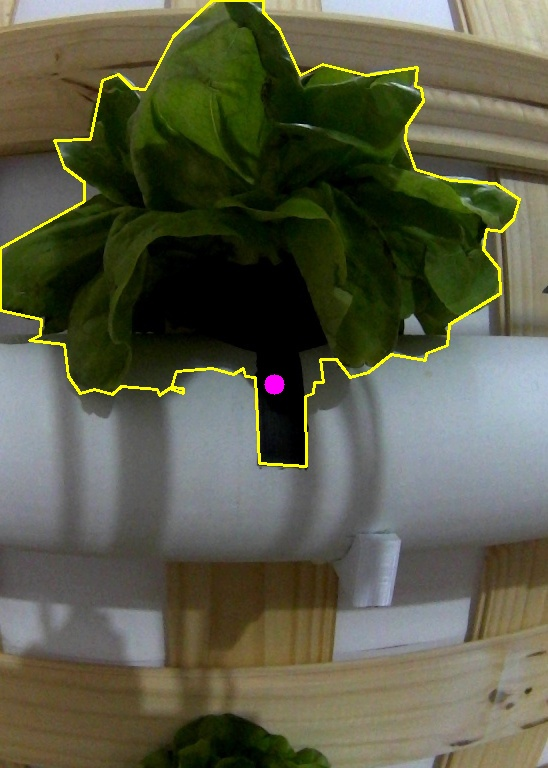
\includegraphics[width=\textwidth]{imagenes/clasificador_6_contornos.jpg}
    \caption{Contornos finales detectados}
\end{subfigure}

\caption{Pipeline completo del sistema de clasificación mostrando las transformaciones sucesivas hasta la extracción de contornos}
\label{fig:pipeline_clasificacion}
\end{figure}